\documentclass{report}
\usepackage[table,xcdraw]{xcolor}
\usepackage{tikz}
\usepackage{fancyhdr}
\usepackage[utf8]{vietnam}
\usepackage{hyperref} % Hyperlink
\usepackage{parskip}
\usepackage[left=2cm,right=2cm,top=2cm,bottom=2cm]{geometry}
\usepackage{minted}
\usetikzlibrary{calc}
\usepackage{titlesec} % Change section font
\usepackage{multirow}
\usepackage{graphicx}
\usepackage{algorithm,algorithmic}
\usepackage{multicol}
\usepackage{setspace}
\usepackage{pdfpages}
\usepackage{lscape}
\usepackage{subfigure}
\usepackage{tabularray}
\usepackage{amsmath}

% ========== [LANGUAGE] ==========
\def\lang{1} % 0 == English, 1 == Vietnamese

\ifnum\lang = 0
    \usepackage[english]{babel}
\fi
% ========== END OF [LANGUAGE] ==========





\begin{document}

% ========== [TITLE PAGE] ==========
\begin{titlepage}

\begin{tikzpicture}[overlay,remember picture]
\draw[line width=4pt]
    ($ (current page.north west) + (1cm,-1cm) $)
    rectangle
    ($ (current page.south east) + (-1cm,1cm) $);
\draw[line width=1.5pt]
    ($ (current page.north west) + (1.2cm,-1.2cm) $)
    rectangle
    ($ (current page.south east) + (-1.2cm,1.2cm) $);
\end{tikzpicture}


\begin{center}
% Upper part of the page
\ifnum\lang = 0
    \textbf{\Large UNIVERSITY OF SCIENCE}\\[0.2cm]
    \textbf{\Large FACULTY OF INFORMATION TECHNOLOGY}\\
\else
    \textbf{\Large TRƯỜNG ĐẠI HỌC KHOA HỌC TỰ NHIÊN}\\
    \textbf{\Large KHOA CÔNG NGHỆ THÔNG TIN}\\
\fi

% University Logo
\begin{figure}[!h]
    \centering
    \includegraphics[width=8cm, height=8cm]{KHTN.png}
\end{figure}

% Title
\rule{\textwidth}{1pt} \\[0.4cm]
{\huge \bfseries BÁO CÁO ĐỒ ÁN - IMAGE PROCESSING}\\[0.4cm]
\textsc{\Large TOÁN ỨNG DỤNG VÀ THỐNG KÊ}
\rule{\textwidth}{1pt} \\[2cm]

% Student name
\begin{center}
    \textbf{\Large HỌ VÀ TÊN: BÙI ĐỖ DUY QUÂN}\\[0.5cm]
    \textbf{\Large MÃ SỐ SINH VIÊN: 21127141}\\[0.5cm]
    \textbf{\Large LỚP: 21CLC02}\\[2cm]
\end{center}

% Advisor name
\begin{center}
    \ifnum\lang = 0
        \textbf{\Large Lecturers: \\[0.2cm]}
    \else
        \textbf{\Large Giảng viên hướng dẫn: \\[0.2cm]}
    \fi
    \Large{Phan Thị Phương Uyên}
\end{center}
\vfill

% Bottom of the page
\ifnum\lang = 0
    \selectlanguage{english} 
\fi
{\large \today}
\end{center}
\end{titlepage}
% ========== END [TITLE PAGE] ==========





% ========== [HEADER AND FOOTER] ==========
\pagestyle{fancy}
\setlength{\headheight}{0.5cm}
\fancyhf{}
\lhead{\textbf{Đồ án 02}}
\rhead{\textbf{Toán ứng dụng và thống kê}}
\ifnum\lang = 0
    \rfoot{Page \thepage}
\else
    \rfoot{Trang \thepage}
\fi
% ========== END [HEADER AND FOOTER] ==========





% ========== [TABLE OF CONTENTS] ==========
\Large
\tableofcontents
\thispagestyle{fancy} % Fix footer and header
\vfill
\pagebreak
% ========== END [TABLE OF CONTENTS] ==========





% ========== [SECTION NUMBERING] ==========
\setcounter{secnumdepth}{10} % Section numbering depth 

\renewcommand\thesection{\arabic{section}} % Section start from 1,2,3...
\renewcommand\thesubsection{\thesection.\arabic{subsection}} % Subsection start from 1,2,3,...
\renewcommand\thesubsubsection{\alph{subsubsection}} 

\titleformat*{\section}{\Large\bfseries}
\titleformat*{\subsection}{\Large\bfseries}
\titleformat*{\subsubsection}{\Large\bfseries}
% ========== END [SECTION NUMBERING] ==========





% ========== [MAIN CONTENT] ==========
\section{YÊU CẦU CỦA ĐỒ ÁN}
\begin{itemize}
    \item Thực hiện các chức năng xử lý ảnh cơ bản như sau: 
        \begin{enumerate}
            \item Thay đổi độ sáng.
            \item Thay đổi độ tương phản.
            \item Lật ảnh (ngang-dọc).
            \item Chuyển đổi ảnh RGB thành ảnh xám/sepia.
            \item Làm mờ/sắc nét ảnh.
            \item Cắt ảnh từ trung tâm theo kích thước.
            \item Cắt ảnh theo khung tròn.
            \item Cắt ảnh theo khung 2 hình ellip chéo nhau (**Nâng cao)
        \end{enumerate}

    \item Các thư viện được sử dụng: \textbf{Numpy}, \textbf{PIL(đọc, ghi ảnh)}, \textbf{matplotlib(hiển thị ảnh)}
\end{itemize}

\section{CÁC CHỨC NĂNG ĐÃ HOÀN THÀNH}
\resizebox{\columnwidth}{!}{%
\begin{tabular}
{|m{0.25\textwidth}|m{0.25\textwidth}|m{0.25\textwidth}|m{0.25\textwidth}|} 
\hline
 STT & Chức năng & Hoàn thành & Kết quả\\   
\hline 
1 &Thay đổi độ sáng&100\% &
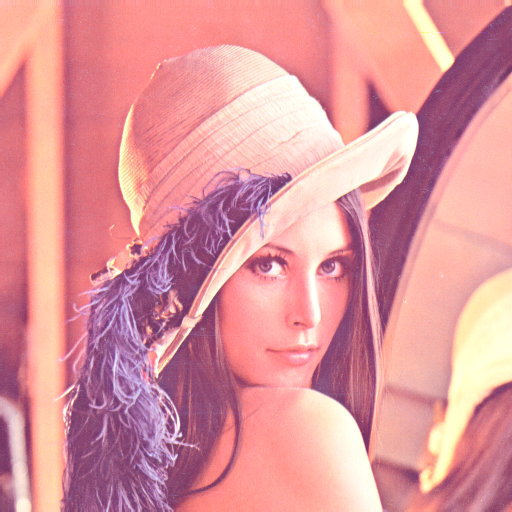
\includegraphics[width=0.25\textwidth, height=3cm, trim=-5cm 0 0 -1cm, keepaspectratio]{image_bright.png} \\  
\hline 
2 &Thay đổi độ tương phản&100\%&
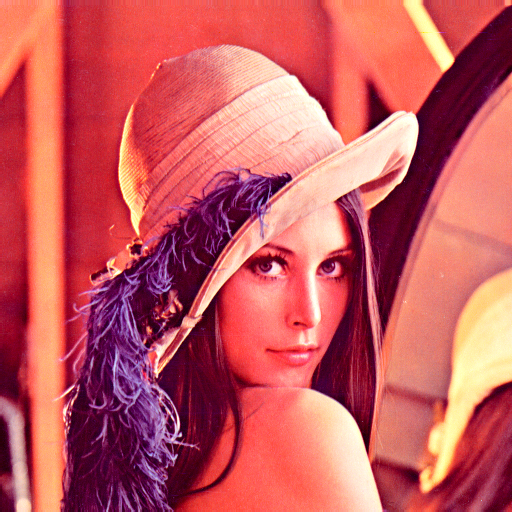
\includegraphics[width=0.25\textwidth, height=3cm, trim=-5cm 0 0 -1cm, keepaspectratio]{image_contrast.png}\\
\hline 
3 &Lật ảnh ngang&100\%&
\includegraphics[width=0.25\textwidth, height=3cm, trim=-5cm 0 0 -1cm, keepaspectratio]{image_flip1.png}\\
\hline 
4 &Lật ảnh dọc&100\%&
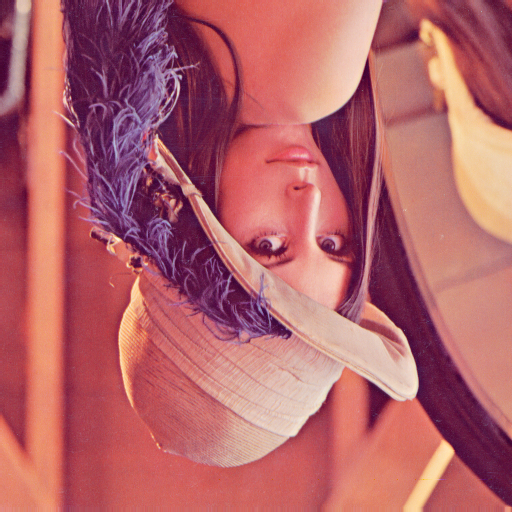
\includegraphics[width=0.25\textwidth, height=3cm, trim=-5cm 0 0 -1cm, keepaspectratio]{image_flip.png}\\
\hline 
\end{tabular} 
}

\newpage
\resizebox{\columnwidth}{!}{%
\begin{tabular}
{|m{0.25\textwidth}|m{0.25\textwidth}|m{0.25\textwidth}|m{0.25\textwidth}|} 
\hline
5 &Ảnh xám&100\%&
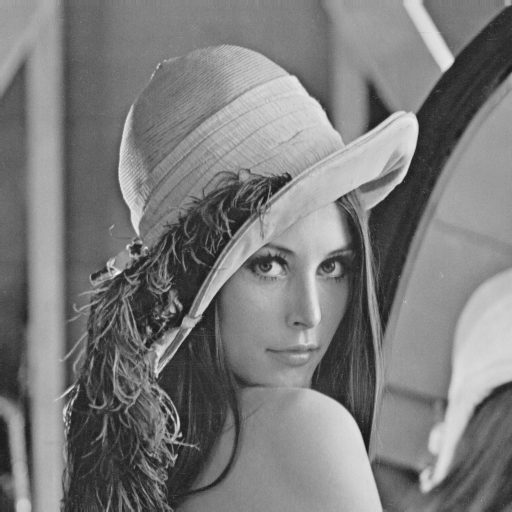
\includegraphics[width=0.25\textwidth, height=3cm, trim=-5cm 0 0 -1cm, keepaspectratio]{image_gray.png}\\
\hline 
6 &Ảnh sepia&100\%&
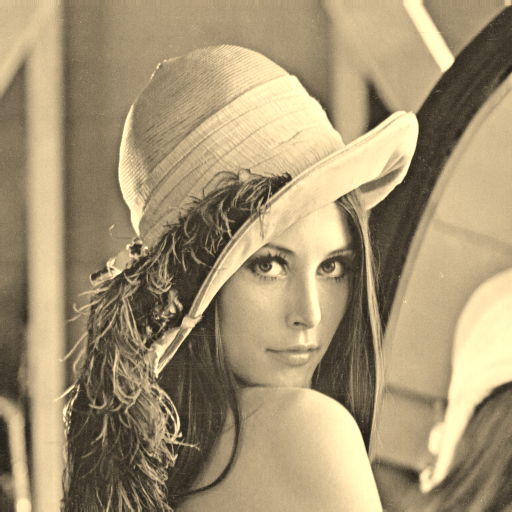
\includegraphics[width=0.25\textwidth, height=3cm, trim=-5cm 0 0 -1cm, keepaspectratio]{image_sepia.png}\\
\hline 
7 &Làm mờ&100\%&
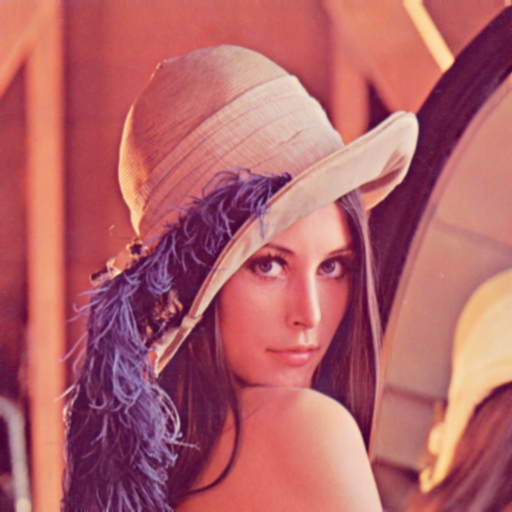
\includegraphics[width=0.25\textwidth, height=3cm, trim=-5cm 0 0 -1cm, keepaspectratio]{image_blur.png}\\
\hline 
8 &Làm sắc nét&100\%&
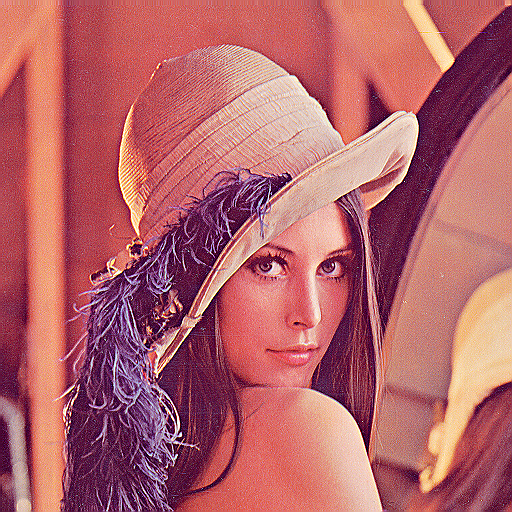
\includegraphics[width=0.25\textwidth, height=3cm, trim=-5cm 0 0 -1cm, keepaspectratio]{image_sharpen.png}\\
\hline 
9 &Cắt từ trung tâm&100\%&
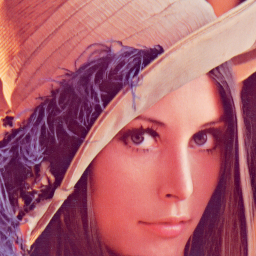
\includegraphics[width=0.25\textwidth, height=3cm, trim=-3cm 0 0 -1cm, keepaspectratio]{image_center.png}\\
\hline 
10 &Cắt khung tròn&100\%&
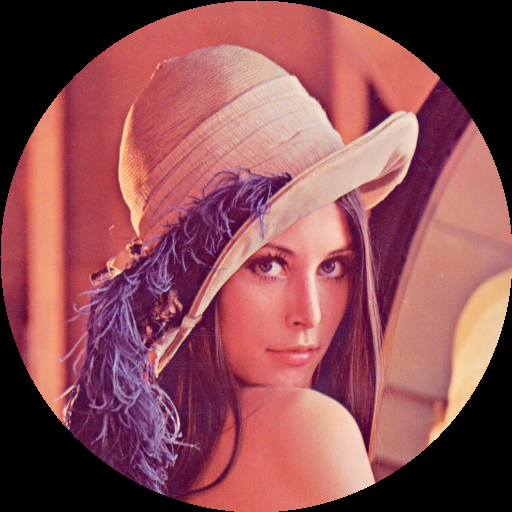
\includegraphics[width=0.25\textwidth, height=3cm, trim=-5cm 0 0 -1cm, keepaspectratio]{image_circle.png}\\
\hline 
11 &Cắt khung 2 ellip chéo nhau&100\%&
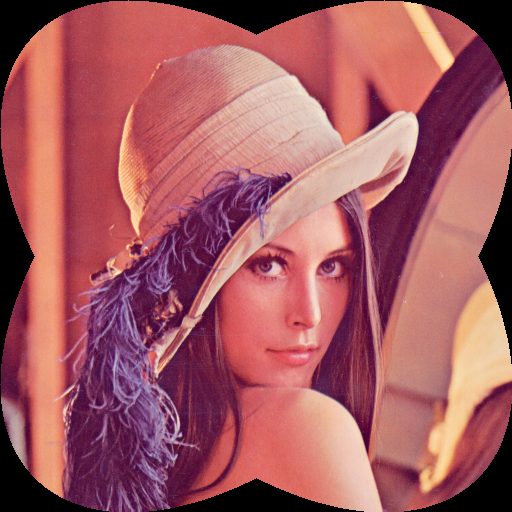
\includegraphics[width=0.25\textwidth, height=3cm, trim=-5cm 0 0 -1cm, keepaspectratio]{image_ellipses.png}\\
\hline 
\end{tabular} 
}
\newpage
\section{CÀI ĐẶT CHƯƠNG TRÌNH}
Chương trình được thiết lập trên tập tin Jupyter Notebook (.ipynb).

\subsection{Kĩ thuật}
Chương trình sẽ được phân thành 2 loại: Hàm hỗ trợ và hàm chức năng.
\subsection{Mô tả các hàm}
\subsubsection{Các hàm hỗ trợ}
\begin{itemize}
    \item Hàm đọc các điểm ảnh.

    \begin{center}
        \textbf{read\_Image(filename)}
    \end{center}
    
    
        \begin{itemize}
            \item Input: Tên file ảnh.
            \item Ouput: 
            \begin{itemize}
                \item Ma trận \textbf{n} chiều các điểm ảnh của bức ảnh đó, với \textbf{n} là số kênh màu của điểm ảnh
                \item Tên của ảnh khi đã tách với phần mở rộng.
            \end{itemize}
            
        \end{itemize}
        
    

    \item Hàm in 2 ảnh song song.
    \begin{center}
        \textbf{show\_Image\_side\_by\_side(image1, image2)}
    \end{center}

        \begin{itemize}
            \item Input: Ma trận điểm ảnh của ảnh 1,  Ma trận điểm ảnh của ảnh 2.
            \item Ouput: Hàm không trả về giá trị, nhưng in 2 ảnh kế nhau ra màn hình.
        \end{itemize}
    
    

    \item Hàm kiểm tra giá trị của từng màu.
    \begin{center}
        \textbf{truncate(image)}
    \end{center}
    
        \begin{itemize}
            \item Input: ma trận màu của các điểm ảnh.
            \item Ouput: Hàm trả về ma trận màu của các điểm ảnh khi đã giới hạn giá trị (nếu ban đầu giá trị màu nào nhỏ hơn 0 thì đưa về bằng 0, còn nếu lớn hơn 255 thì sẽ đưa về bằng 255).
        \end{itemize}

    \item Hàm chọn chức năng.
    \begin{center}
        \textbf{Menu(Feature\_Name)}
    \end{center}
        \begin{itemize}
            \item Input: Mảng tên các chức năng.
            \item Output: Lựa chọn của người dùng (số nguyên).
        \end{itemize}

   \item Hàm xử lý ảnh.
   \begin{center}
       \textbf{process(image, Feature)}
   \end{center}
        \begin{itemize}
            \item Input: Ma trận màu các điểm ảnh, chức năng sẽ thực hiện.
            \item Output: Ma trận màu các điểm ảnh sau khi đã xử lý theo chức năng.
        \end{itemize}

    \item Hàm lưu ảnh.
    \begin{center}
        \textbf{save\_Image(image, filename, Feature)}
    \end{center}
        \begin{itemize}
            \item Input: Ma trận màu các điểm ảnh, tên của ảnh được xử lý, tên chức năng.
            \item Output: Hàm không trả về giá trị, nhưng sẽ thực hiện lưu ảnh kết quả với tên tập tin là: "\textbf{(tên ảnh)\_(tên chức năng).png}"
        \end{itemize}
\end{itemize}

\subsubsection{Các hàm thực hiện chức năng}
\textit{Trong phần này sẽ đưa ra ý tưởng, mô tả các hàm chức năng}
    \begin{enumerate}
        \item Thay đổi độ sáng của ảnh.
            \begin{itemize}
                \item Ý tưởng: ý tưởng của việc thay đổi độ sáng của ảnh chính là việc cộng vào giá trị màu của các điểm ảnh với cùng 1 giá trị nào đó. Nếu giá trị được cộng vào là giá trị âm (< 0) thì sẽ làm cho màu của ảnh tối đi, ngược lại sẽ làm cho ảnh sáng hơn.
        
                \item Mô tả hàm:
                \begin{center}
            \textbf{bright\_Image(image, brightness)}
                \end{center}
        
                    \begin{itemize}
                        \item Input: Ma trận màu các điểm ảnh, giá trị cộng thêm để thay đổi độ sáng.
                        \item Ouput: Ma trận màu các điểm ảnh sau khi được công thêm giá trị độ sáng.
                        \item Cách hoạt động của hàm này đó chính là tận dụng thư viện \textbf{numpy} hỗ trợ cho việc thực hiện phép cộng giữa 1 ma trận và 1 số. Như vậy, ta chỉ cần thực hiện phép cộng bình thường giữa ma trận điểm ảnh và giá trị thay đổi độ sáng, kết trả sẽ là từng  giá trị màu của điểm ảnh sẽ được thay đổi 1 lượng đúng bằng giá trị thay đổi. Đồng thời chúng ta cũng phải kiểm soát giá trị của các màu trong điểm ảnh vì có thể giá trị có thể bị vượt quá đoạn [0, 255]. Vì vậy, khi giá trị màu vượt quá 255 thì sẽ gán về 255, còn giảm nhỏ hơn 0 thì sẽ gán giá trị lên bằng 0.
                    \end{itemize}
                \pagebreak
                \item Hình ảnh kết quả:
                \begin{figure}[!h]
                    \centering
                    \includegraphics[width=\textwidth, keepaspectratio]{bri.png}
                    \caption{Tăng độ sáng của ảnh với giá trị là 50}
                \end{figure}
            \end{itemize}
            
        \item Thay đổi độ tương phản.
            \begin{itemize}
                \item Ý tưởng: ý tưởng của việc thay đổi độ tương phản chính là tăng giảm sự chênh lệch giữa cường độ tối đa và tối thiểu của điểm ảnh trong 1 bức hình. Như vậy, để tăng giảm sự chênh lệch thì ta cần nhân 1 lượng giá trị vào các giá trị màu của điểm ảnh.

                \item Mô tả hàm:
                 \begin{center}
            \textbf{contrast\_Image(image, ContrastValue)}
                \end{center}

                    \begin{itemize}
                        \item Input: Ma trận của các điểm ảnh, giá trị tương phản muốn thay đổi.
                        \item Output: Ma trận của các điểm ảnh sau khi được nhân 1 lượng giá trị.
                        \item Cách thức hoạt động của hàm:
                            \begin{itemize}
                                \item Để thay đổi sự tương phản của ảnh, ta sẽ cần thay đổi giá trị lớn nhất và nhỏ nhất cường độ điểm ảnh, tuy nhiên nếu chỉ thay đổi giá trị giữa các điểm ảnh thì sẽ không làm thay đổi gì nhiều ở bức ảnh. Vì vậy chúng ta sẽ cần tính hệ số chỉnh độ tương phản với công thức:
                                \begin{center}
                                    $F = [259*(255+C)]\div[255*(259-C)]$
                                \end{center}
                                Với C là giá trị mức độ của độ tương phản khi truyền vào hàm $(C \in [-255; 255])$.
    
                                \item Từ đây mới thực hiện điểu chỉnh độ tương phản. Mỗi màu sẽ được điều chỉnh theo công thức sau:
                                \begin{center}
                                    $NewA = F * (A - 128) + 128$
                                \end{center}
                                Với \textit{A} là giá trị hiện tại của từng màu của điểm ảnh và \textit{NewA} là giá trị mới của màu đó sau khi thực hiện tính toán.
    
                                \item Cũng cần lưu ý rằng phải kiểm soát giá trị của từng màu để giá trị của màu luôn thuộc đoạn [0;255] sau khi thực hiện điều chỉnh.
                            \end{itemize}
                    \end{itemize}
                \item Hình ảnh kết quả:
                \begin{figure}[!h]
                    \centering
                    \includegraphics[width=\textwidth, keepaspectratio]{contr.png}
                    \caption{Tăng độ tương phản của ảnh với giá trị là 50}
                \end{figure}
            \end{itemize}
        \item Lật ảnh (ngang-dọc).
            \begin{itemize}
                \item Ý tưởng: Bản chất của một hình RGB được tổ chức dưới dạng là ma trận của các điểm ảnh. Từ đó có thể thấy, để có thể xoay hình ngang hay dọc thì chúng ta sẽ thực hiện đảo ngược thứ tự của các điểm ảnh (đảo ngược các hàng hoặc đảo ngược các cột).

                \pagebreak
                \item Mô tả hàm:
                 \begin{center}
            \textbf{flip\_Image(image, dir)}
                \end{center}
                \begin{itemize}
                    \item Input: Ma trận điểm ảnh, chiều xoay của hình (số nguyên: 0-xoay theo trục tung, 1-xoay theo trục hành).
                    \item Output: Ma trận điểm ảnh sau khi đã đảo ngược các phần tử theo chiều quay được truyền vào hàm.
                    \item Cách thức hoạt động của hàm:
                        \begin{itemize}
                            \item Như đã nêu ở phần tử, thực hiện lật ảnh ngang hoặc dọc bản chất chính là đảo ngược thứ tự của các phần tử trong mả trận.
                            \item Giả sử nếu ta có ma trận điểm ảnh, với mỗi phần tử đại diện cho 1 điểm ảnh chứa các giá trị R-G-B:
                            \begin{center}
                                $
                                \begin{bmatrix}
                                a & b & c\\
                                d & e & f\\
                                \end{bmatrix}
                                $
                            \end{center}
                            \item Như vậy, khi thực hiện lật ảnh ngang, chúng ta sẽ đảo thứ tự các phần tử theo cột, và kết quả của ma trận đó sẽ là:
                            \begin{center}
                                $
                                \begin{bmatrix}
                                a & b & c\\
                                d & e & f\\
                                \end{bmatrix}
                                \to
                                \begin{bmatrix}
                                c & b & a\\
                                f & e & d\\
                                \end{bmatrix}
                                $
                            \end{center}
                            \item Ngược lại, thực hiện lật ảnh dọc sẽ đảo ngược thứ tự các phần tử thẹo hàng thì ta được kết quả:
                             \begin{center}
                                $
                                \begin{bmatrix}
                                a & b & c\\
                                d & e & f
                                \end{bmatrix}
                                \to 
                                \begin{bmatrix}
                                d & e & f\\
                                a & b & c\\
                                \end{bmatrix}
                                $
                            \end{center}
                            \item Để thực hiện đảo ngược thứ tự thì ta sẽ cần dùng kĩ thuật \textbf{Slicing}, giúp truy xuất phần tử theo chiều ngược lại. Ngoài ra có thể sử dùng hàm có sẵn trong thư viện
                            \textbf{numpy} và đó là hàm \textbf{numpy.flip}
                        \end{itemize}
                \end{itemize}
                \pagebreak
                \item Hình ảnh kết quả:
                \begin{figure}[!h]
                    \centering
                    \includegraphics[width=\textwidth, keepaspectratio]{flip.png}
                    \caption{Lật ảnh dọc}
                \end{figure}
                \begin{figure}[!h]
                    \centering
                    \includegraphics[width=\textwidth, keepaspectratio]{flip1.png}
                    \caption{Lật ảnh ngang}
                \end{figure}
            \end{itemize}
        \pagebreak
        \item Chuyển đổi ảnh RGB thành ảnh xám.
            \begin{itemize}
                \item Ý tưởng: Bản chất của ảnh màu xám chính là các giá trị màu trong điểm ảnh chỉ dùng để thể hiện độ sáng chứ không thể hiện màu sắc của ảnh. Giá trị của độ sáng sẽ nằm trong đoạn [0; 255] với 0 là màu đen và 255 sẽ là màu trắng. Như vậy, trong ảnh màu RGB, mỗi điểm ảnh sẽ chứa giá trị 3 màu, và để chuyển thành ảnh màu xám thì ta phải cần lấy giá trị độ sáng trung bình giữa 3 màu này cho mỗi điểm ảnh.

                \item Mô tả hàm:
                \begin{center}
                \textbf{convert\_To\_Gray(image)}
                \end{center}
                    \begin{itemize}
                        \item Input: Ma trận điểm ảnh của hình.
                        \item Output: Ma trận điểm ảnh sau khi chuyển đổi thành màu xám.
                        \item Cách thức hoạt động của hàm:
                        \begin{itemize}
                            \item Để tìm được giá trị độ sáng trung bình giữa 3 màu thì có rất nhiều cách, và ở trong hàm này sẽ được cài đặt theo \textbf{Phương pháp độ sáng (Luminosity Method)}.
                            \item Với mỗi điểm ảnh giờ đây chỉ còn 1 giá trị để biểu thị về độ sáng, chính vì vậy giá trị mới của điểm ảnh sẽ là tổng của 3 màu cùng với hệ số của từng màu, tức là:
                            \begin{center}
                                $Gray = 0.299 * R + 0.587 * G + 0.114 * B$    
                            \end{center}
                            \item Những hệ số này có được thông qua nhiều lần nghiên cứu và phân tích sâu thì hệ số này ra đời,và rất phù hợp trong việc chuyển đổi từ ảnh màu thành ảnh xám.
                            \item Theo như công thức ở trên, chúng ta sẽ thực hiện nhân ma trận nhờ phương pháp \textbf{broadcasting} để mỗi màu của điểm ảnh đều được nhân với hệ số của nó. Sau đó thực hiện phép cộng tổng theo chiều trong cùng tức là cộng các giá trị của 3 màu trong 1 điểm ảnh để được 1 giá trị chung, biểu thị cho độ sáng của điểm ảnh đó.
                        \end{itemize}
                    \end{itemize}
                \pagebreak
                \item Hình ảnh kết quả:
                \begin{figure}[!h]
                    \centering
                    \includegraphics[width=\textwidth, keepaspectratio]{gra.png}
                    \caption{Kết quả chuyển từ ảnh màu sang ảnh xám}
                \end{figure}
            \end{itemize}
        \item Chuyển đổi ảnh RGB thành ảnh sepia.
            \begin{itemize}
                \item Ý tưởng: Để chuyển đổi từ ảnh màu thành ảnh sepia thì ta cần chuyển đổi giá trị 3 màu R-G-B về với thang màu sepia dựa theo công thức đã được có sẵn.

                \item Mô tả hàm:
                    \begin{center}
                        \textbf{convert\_To\_Sepia(img)}
                    \end{center}
                    \begin{itemize}
                        \item Input: Ma trận điểm ảnh của hình.
                        \item Output: Ma trận điểm ảnh của hình sau khi các màu của điểm ảnh đã được chuyển đổi về thang màu sepia.
                        \item Cách thức hoạt động của hàm:
                            \begin{itemize}
                                \item Để chuyển đổi giữa ảnh màu thành ảnh sepia thì mỗi màu của điểm ảnh sẽ được nhận giá trị mới theo công thức sau:
                                \begin{center}
                                NewRed = 0.393 * R + 0.769 * G + 0.189 * B\\
                                    
                                NewBlue = 0.349 * R + 0.686 * G + 0.168 * B\\
                                    
                                NewGreen = 0.272 * R + 0.534 * G + 0.131 * B 
                                \end{center}
                                \item Sau khi tính các giá trị mới cho cho từng màu của điểm ảnh, ta sẽ xét ở mỗi màu của điểm ảnh, nếu giá trị của màu vượt quá 255 thì màu sẽ nhận giá trị là 255, còn nếu vẫn nhỏ hơn 255 thì sẽ giữ nguyên giá trị của màu đó.
                                \item Dựa theo công thức đã cho ở trên, công việc tính toán được cụ thễ hoá bài toán nhân ma trận giũa ma trận điểm ảnh và ma trận giá trị của các hệ số cho từng màu. Chúng ta có thể sử dụng toán tử \textbf{@} để thực hiện nhân ma trận từng điểm ảnh với các hệ số và sau đó tính tổng để cho ra giá trị của từng màu. Ngoài ra, thư viện \textbf{numpy} cũng hỗ trợ việc tính toán này qua hàm \textbf{numpy.dot}
                            \end{itemize}
                    \end{itemize}
                \item Hình ảnh kết quả:
                \begin{figure}[!h]
                    \centering
                    \includegraphics[width=\textwidth, keepaspectratio]{sep.png}
                    \caption{chuyển từ ảnh màu sang ảnh sepia}
                \end{figure}
            \end{itemize}
        \item Làm mờ và làm sắc nét ảnh.
            \begin{itemize}
                \item Ý tưởng: ý tưởng của việc làm mờ hay làm sắc nét ảnh đó là mức độ chia sẻ màu giữa các điểm ảnh với nhau trong hình. Mỗi điểm ảnh sẽ được tính bằng cách cộng thêm các giá trị trọng số của tất cá các điểm ảnh lân cận với điểm ảnh đó.

                \pagebreak
                \item Mô tả hàm:
                \begin{center}
                    \textbf{convert\_To\_Blur(image)\\
                    convert\_To\_Sharpen(image)}
                \end{center}
                \begin{itemize}
                    \item Input: Ma trận điểm ảnh của hình.
                    \item Output: Ma trận điểm ảnh sau khi đã được chuyển đổi thành hình mờ (hoặc hình sắc nét).
                    \item Việc làm mờ hay làm sắc nét của 1 hình là quá trình \textbf{"tích chập" (convolution)} giữa ma trận hình và ma trận \textbf{"cửa sổ" (kernel)}. Nói 1 cách dễ hiểu, với mỗi điểm ảnh sẽ được cộng thêm 1 lượng trọng số của các điểm ảnh lân cận, trọng số đó chính là \textbf{Kernel}. Trọng số này sẽ thể hiện cho tỉ lệ đóng góp màu của 1 điểm ảnh trong 1 không gian các điểm ảnh nhất định.
    
                    \item Để có thể tình toán chính xác nhất thì giá trị của ma trận Kernel phải chính xác. Thông thường trong xử lý làm mờ ảnh và làm rõ nét thì sẽ lựa chọn lần lượt các kernel là  \textbf{Gaussian blur(3x3)} và \textbf{Sharpen(3x3)}. Tuỳ vào việc xử lý làm ảnh mờ hay làm rõ nét ảnh mà chọn Kernel phù hợp. Các Kernel này có giá trị là
                    
                    \begin{center}
                        \begin{tabular}{c@{\hspace{1cm}}c}
                        $BlurK =  \dfrac{1}{16}
                        \begin{bmatrix}
                            1 & 2 & 1\\
                            2 & 4 & 2\\
                            1 & 2 & 1
                        \end{bmatrix} $&                   
                        $SharpenK =\begin{bmatrix}
                            0 & -1 & 0\\
                            -1 & 5 & -1\\
                            0 & -1 & 0
                        \end{bmatrix}$
                         \end{tabular}
                    \end{center}
    
                    \item Như vậy, với kích thước của Kernel là 3x3, mỗi điểm ảnh sẽ là điểm trung tâm của ma trận 3x3 với các điểm lân cận. Giá trị mới của điểm ảnh là tổng của các giá trị điểm ảnh lân cận đã được nhân với từng giá trị tương ứng của Kernel (bao gồm cả điểm ảnh trung tâm). Có thể khái quát công thức tính giá trị mới của 1 điểm ảnh với ma trận Kernel 3x3 như sau:
                    \[Pixel(i,j) =\sum_{n=i-1}^{i+1} \sum_{m=j-1}^{j+1} Pixel(n,m) * Kernel(n,m)\]
                    
                    \item Một lưu ý đó là để dễ dàng cho việc tính toán và cài đặt hàm, chúng ta sẽ không xử lý các điểm ảnh thuộc hàng đầu, hàng cuối, cột đầu, cột cuối của ảnh đối với ma trận Kernel 3x3 vì các điểm ảnh của vị trí này không nằm trong ma trận 3x3 nào cả. Ngoài ra, để thuận tiện cho việc tính toán thì có thể cài đặt chương trình bằng cách sử dụng hàm do thư viện \textbf{numpy} cung cấp đó là \textbf{numpy.convolve}.
                \end{itemize}
                \item Hình ảnh kết quả:
                \begin{figure}[!h]
                    \centering
                    \includegraphics[width=\textwidth, keepaspectratio]{blur.png}
                    \caption{Làm mờ ảnh}
                \end{figure}

                \begin{figure}[!h]
                    \centering
                    \includegraphics[width=\textwidth, keepaspectratio]{sharp.png}
                    \caption{Làm rõ nét ảnh}
                \end{figure}
            \end{itemize}
    \end{enumerate}

\newpage
\section{THỰC THI CHƯƠNG TRÌNH CHÍNH}
\subsection{Các thông tin đầu vào được yêu cầu}
\begin{itemize}
    \item Khi bắt đầu chạy chương trình, người dùng sẽ được yêu cầu nhập các thông tin đầu vào như sau:
        \begin{itemize}
            \item \textbf{Tên tập in ảnh} (bao gồm đuôi file: png, jpg) và tập tin ảnh phải cùng chung thư mục với tập tin chương trình.
            \item \textbf{Số lượng cụm màu}. Số lượng cụm màu càng lớn, chương trình thực thi có thể sẽ chậm hơn, tốt nhất số cụm màu từ [3-256] để đảm bảo chất lượng hình sau khi nén.
            \item \textbf{Số lượng vòng lặp.}
            \item \textbf{Loại khởi tạo các mảng màu trung tâm}: \textbf{'random'} hoặc \textbf{'in\_pixels'}. Người dùng cần nhập \underline{đúng tên của loại khởi tạo} thì chương trình mới được thực thi.
            \item \textbf{Định dạng để lưu hình sau khi nén}: \textbf{pdf} và \textbf{png}. Người dùng cần \underline{nhập đúng tên định dạng} để chương trình chạy đúng.
        \end{itemize}
    \item Sau khi chạy và nhập đúng, đủ các thông tin đầu vào thì chương trình sẽ thực thi nén ảnh. Nén ảnh xong, tập tin ảnh mới sẽ được lưu với tên \textbf{Result.a} với a là định dạng mà người dùng muốn lưu khi nhập ban đầu.Đồng thời dưới chương trình cũng sẽ xuất ra màn hình 2 loại hình: ảnh gốc và ảnh sau khi nén để cho người dùng dễ so sánh sự thay đổi.
    \end{itemize}
\subsection{Hình ảnh khi chạy chương trinh}
\subsubsection{Nhập thông số đầu vào}
\begin{figure}[ht!]
     \begin{center}
%
        \subfigure[Tên tập tin ảnh]{%
            \label{fig:first}
            \includegraphics[width=0.5\textwidth]{i1.png}
        }%
        \subfigure[Số cụm]{%
           \label{fig:second}
           \includegraphics[width=0.5\textwidth]{i2.png}
        }\\ %  ------- End of the first row ----------------------%
        \subfigure[Số vòng lặp]{%
            \label{fig:third}
            \includegraphics[width=0.5\textwidth]{i5.png}
        }%
        \subfigure[Loại khởi tạo màu trung tâm]{%
            \label{fig:fourth}
            \includegraphics[width=0.5\textwidth]{i3.png}
        }\\%
        
        \subfigure[Định dạng tập tin kết quả]{%
            \label{fig:fourth}
            \includegraphics[width=0.5\textwidth]{i4.png}
        }%
%
    \end{center}
\end{figure}
\subsubsection{Kết quả của chương trình}
\begin{figure}[ht!]
     \begin{center}
%
        \subfigure[Vị trí của tập tin kết quả]{%
            \label{fig:first}
            \includegraphics[width=0.5\textwidth]{result_image.png}
        }%
        \subfigure[Kết quả in ra màn hình]{%
           \label{fig:second}
           \includegraphics[width=0.5\textwidth]{result_output.png}
        }\\ %  ------- End of the first row ----------------------%
    \end{center}
\end{figure}
\section{NHẬN XÉT CÁC TRƯỜNG HỢP CỦA THUẬT TOÁN}
\begin{itemize}
    \item Trong phần này sẽ thực hiện chạy chương trình với số lượng màu nén xuống lần lượt là: 3, 5, 7.
    \item Trong 3 trường hợp màu này, số vòng lặp cao nhất sẽ được khai báo là 100.
    \item Hình được sử dụng trong lần kiểm thử này có kích thước 600x800.
    \item Cách khởi tạo các màu trung tâm sẽ là 'random'.
    \item Thông số của máy tính chạy chương trình: 11th Gen Intel(R) Core(TM) i5-1135G7 @ 2.40GHz   1.38 GHz 16.0 GB RAM
\end{itemize}

\begin{enumerate}
\newpage
\item Đối với hình khi nén xuống còn 3 màu, chắc chắn hình ảnh sẽ khác rất nhiều so với ảnh gốc vì chỉ còn 3 màu chính: xanh lá đậm, xanh lá nhạt, xanh dương nhạt. Các hình ảnh cơ bản nhất như mây, hoa hay mặt nước là không thể nhận ra được. Các đường nét của các sự vật cũng nhìn rất đơn giản.
\begin{figure}[!h]
    \centering
    \includegraphics[width=\textwidth]{3.png}
    \caption{Kết quả K = 3}
\end{figure}

\newpage
\item Đối với hình khi còn 5 màu thì số lượng màu đã được tăng thêm, giờ đây ta có thể nhận thấy màu trắng của mây và màu xanh dương đậm ở vùng trời trên cùng. Ở màu này cho chúng ta nhận biết một chút về bầu trời, tuy nhiên đường nét của sự vật vẫn chưa rõ nét.
\begin{figure}[!h]
    \centering
    \includegraphics[width=\textwidth]{5.png}
    \caption{Kết quả K = 5}
\end{figure}

\newpage
\item Hình khi có 7 màu thì không thấy nhiều thay đổi lớn, có thêm 2 màu nữa làm rõ màu hoa vàng và phần bóng của cây ở mặt mước. Tuy đường nét vẫn cơ bản nhưng các màu cũ được tô thêm nhiều hơn, giúp người dùng hình dung được hình tốt hơn.
\begin{figure}[!h]
    \centering
    \includegraphics[width=\textwidth]{7.png}
    \caption{Kết quả K = 7}
\end{figure}
\end{enumerate}

\section{KẾT LUẬN}
\begin{itemize}
    \item Trong nhiều lần chạy các trường hợp khác về số lượng cụm giảm và số lần lặp tối đa thì có thể nhận xét như sau:
    \begin{itemize}
        \item Số cụm nhỏ và số lần lặp nhỏ: Hình sẽ rất khó nhìn và gần như không thể nhận biết được so với hình gốc.
        \item  Số cụm lớn và số lần lặp nhỏ: Hình xử lý nhanh, có thể nhận biết được hình với ảnh gốc, nhưng có nhiều điểm ảnh lỗi.
        \item Số cụm nhỏ và số lần lặp lớn: Hình xử lý nhanh, người dùng có thể hình dung sơ được hình nhưng vẫn rất sơ sài màu.
        \item  Số cụm nhiều và số lần lặp nhiều: Hình sát với hình gốc, ít thấy điểm ảnh sai, nhưng thời gian xử lý lâu.
        \end{itemize}
    \item Có thể thấý, thuật toán K-Means thích hợp để có thể sử dụng trong việc nén ảnh xuống số màu nhất định. Tốc độ chạy của thuật toán này tối ưu nhất sẽ là việc lựa chọn số cụm cần giảm xuống và điều kiện dừng để người dùng đạt được hình có thể nhận biết tốt nhất có thể.
    
\end{itemize}
\section{TÀI LIỆU THAM KHẢO}
\begin{itemize}
    \item 
    \href{https://www.youtube.com/watch?v=uLs-EYUpGAw&t=524s}{Pseudo code K-Means}

    \item
    \href{https://www.youtube.com/watch?v=4b5d3muPQmA}{Giải thích K-Means}
    
    \item \href{https://numpy.org/doc/stable/user/basics.broadcasting.html}{Kĩ thuật Broadcasting}

    \item \href{https://stackoverflow.com/questions/1408311/numpy-array-slice-using-none}{Slicing với phần tử None}

    \item \href{https://www.researchgate.net/publication/321502735_Centroid_Update_Approach_to_K-Means_Clustering}{Công thức toán học và các phương pháp cập nhật điểm màu trung tâm}

    \item \href{https://numpy.org/doc/stable/user/index.html#user}{Tài liệu các hàm trong thư viện numpy}

    \item \href{https://matplotlib.org/stable/api/_as_gen/matplotlib.pyplot.imshow.html}{Thư viện matplotlib hỗ trợ xuất ảnh và lưu ảnh}

    \item \href{https://pillow.readthedocs.io/en/stable/reference/Image.html}{Thư viện Pillow hỗ trợ đọc ảnh}
    
\end{itemize}
% ========== END [MAIN CONTENT] ==========
\end{document}